\documentclass{standalone}
\usepackage{tikz}
\usetikzlibrary{arrows.meta, calc, patterns, decorations.pathmorphing, decorations.markings, math}

\begin{document}
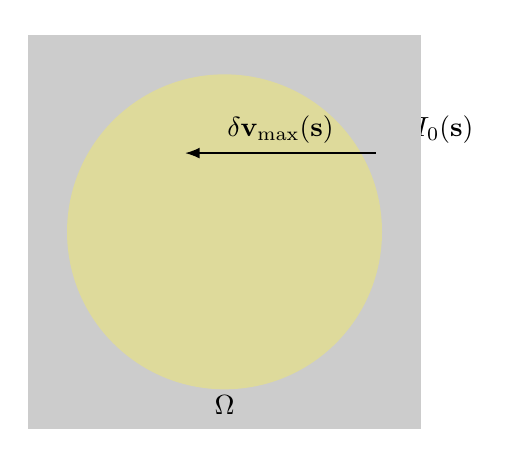
\begin{tikzpicture}[
    dot/.style={circle, fill=black, minimum size=4pt, inner sep=0},
    arrow/.style={-Latex}]
    
    % Gradient nodes
    \node[dot] (grad0) at (2,1) {};
    \node[dot] (grad1) at (1.7,1.7) {};
    \node[dot] (grad2) at (1,2) {};
    \node[dot] (grad3) at (0.5,0.5) {};
    \node[dot] (grad4) at (-1,1.5) {};
    
    % Gradient labels
    \node[above right] at (grad0) {$\nabla I_0(\mathbf{s})$};
    \node[above] at (grad1) {$\nabla I_1(\mathbf{s})$};
    \node[above] at (grad2) {$\nabla I_2(\mathbf{s})$};
    \node[below] at (grad3) {$\nabla I_3(\mathbf{s})$};
    \node[above left] at (grad4) {$\nabla I_4(\mathbf{s})$};
    
    % Arrow between gradients
    \draw[arrow] (grad0) -- (grad1);
    \draw[arrow, dashed] (grad0) -- (grad2);
    \draw[arrow] (grad0) -- (grad4);
    
    % Circle for region D(s)
    \draw[line width=1pt] (0,0) circle (2cm);
    
    % Region label
    \node at (0, -1.3) {$D(\mathbf{s})$};
    
    % Domain Omega
    \fill[gray!40] (-2.5,-2.5) rectangle (2.5,2.5);
    \fill[olive!30!white] (0,0) circle (2cm);
    \node at (0, -2.2) {$\Omega$};
    
    % Maximum vector label
    \draw[line width=0.5pt, arrow] (grad0) -- (-0.5,1) node[midway, above, sloped] {$\delta \mathbf{v}_{\max}(\mathbf{s})$};
    
\end{tikzpicture}
\end{document}